The following sections aims to describe the integration and integration testing sequence of the different components and subsystems of \emph{PowerEnJoy}. From now on the following notation will be used: an arrow going from component C1 to component C2 points out that C2 is necessary to C1 to work properly.

\subsection{Software Integration Sequence}
The components of each subsystem are tested starting from the most to the least independent one.

%Ricordarsi che il car status manager offre una interfaccia menre il payment gateway ne usa una.

\subsection{Subsystem Integration Sequence}
The integration sequence of the high-level subsystems is described in Figure \ref{h_level_subsys} and Table \ref{subsys_int}.

\begin{figure}[H]
\begin{center}
		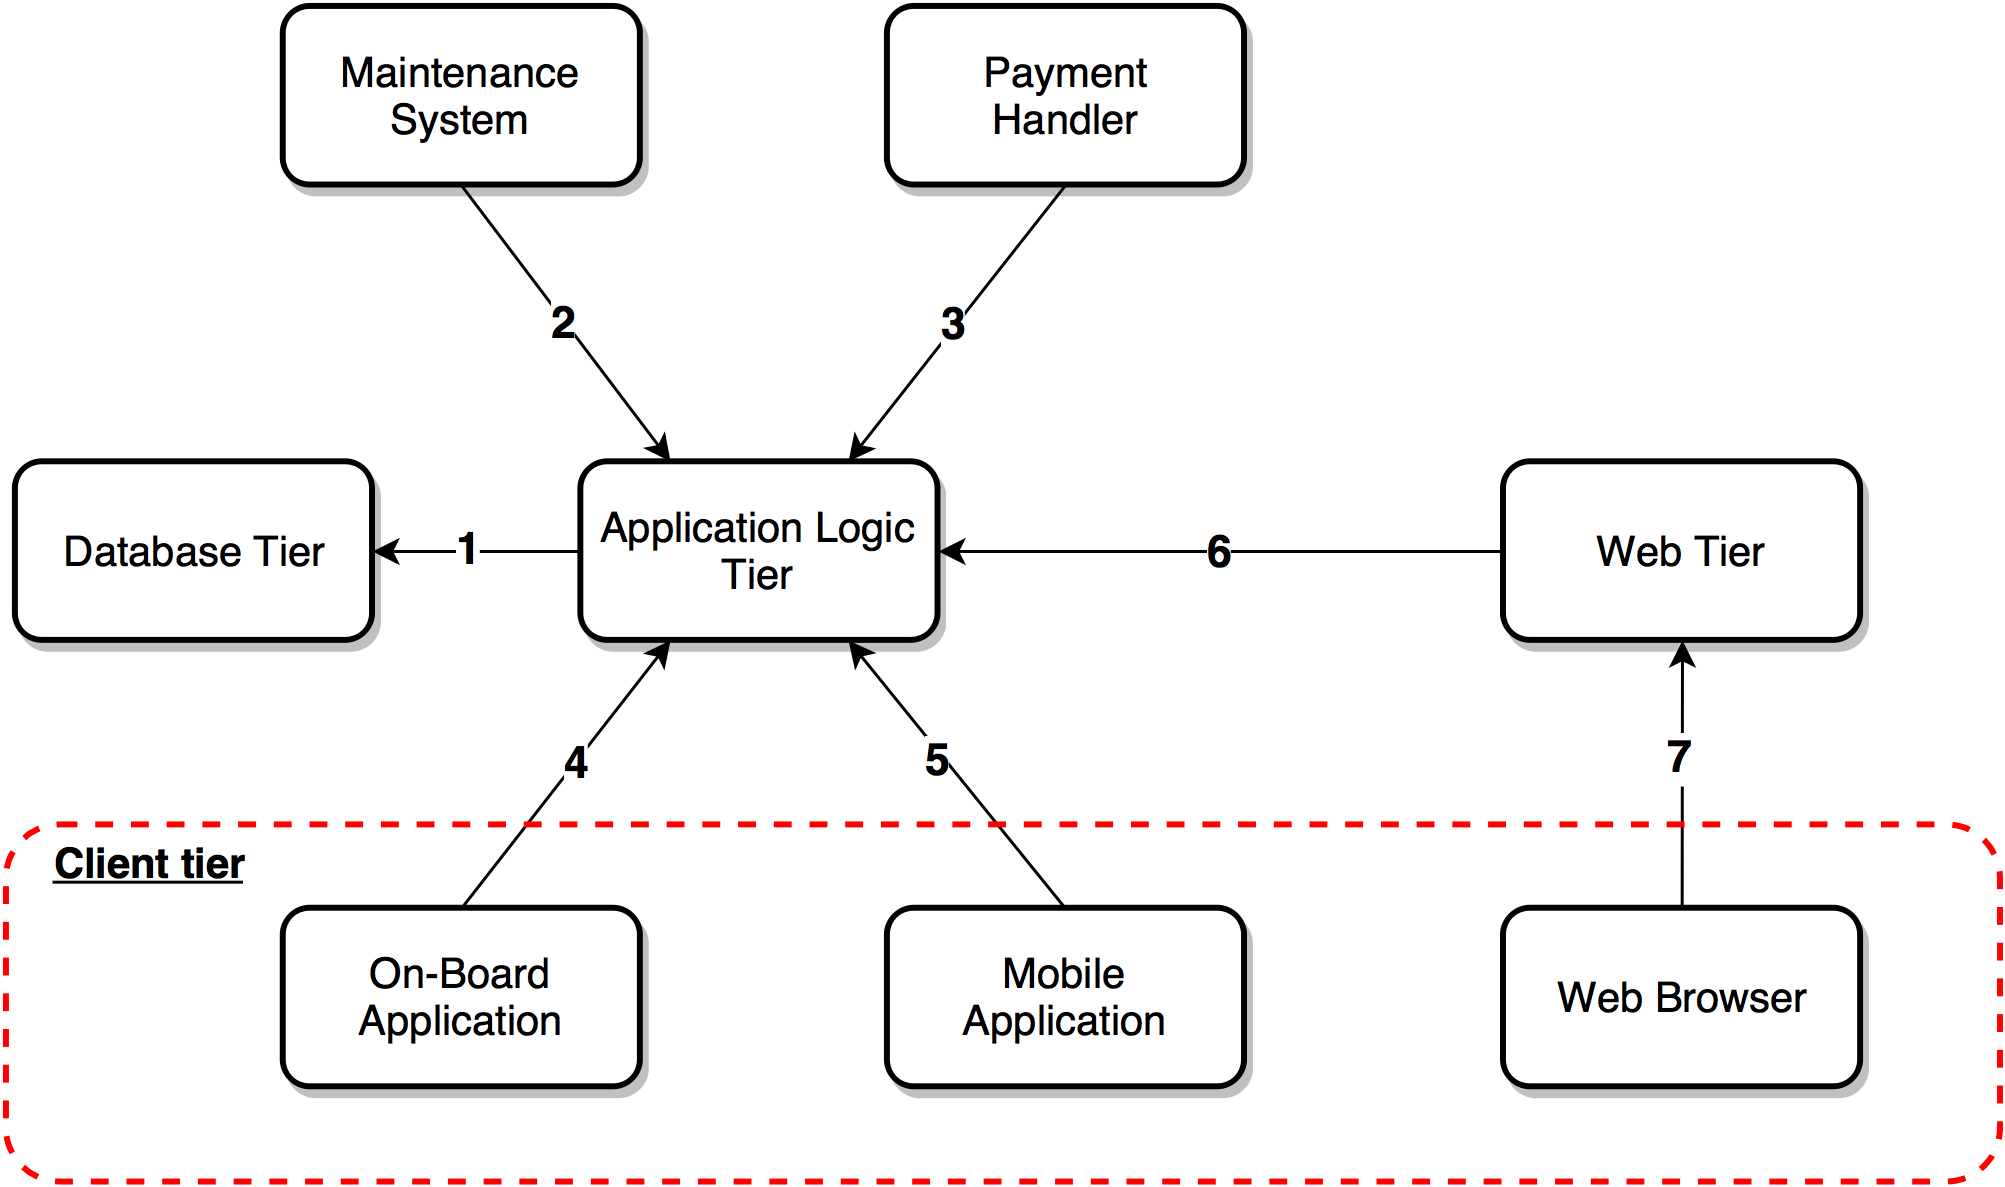
\includegraphics[width=\textwidth]{./integration_strategy/diagrams/h_level_subsys.png}
		\caption{Diagram representing the order of the subsystems integration.}
		\label{h_level_subsys}
\end{center}
\end{figure}

\begin{table}[H]
\begin{center}
\begin{tabular}{p{0.2\textwidth} | p{0.4\textwidth} | p{0.4\textwidth}}
\hline
\textbf{N.} & \textbf{Subsystem} & \textbf{Integrates with} \\
\hline
SI1 & Application Logic Tier & Database Tier \\
\hline
SI2 & Mobile Application & Application Logic Tier \\
\hline
SI3 & On-Board Application & Application Logic Tier \\
\hline
SI4 & Web Tier & Application Logic Tier \\
\hline
SI5 & Web Browser & Web Tier \\
\hline
\end{tabular}
\end{center}
\caption{Integration order of the subsystems described in Section \ref{elems_int}.}
\label{subsys_int}
\end{table}

%MOTIVAZIONI DELLA SCELTA
%Prima il livello dati e poi la business logic prima dei client. La business logic deve funzionare per avere dei
%client altrettanto funzionanti.
%Inoltre notare come prima del web tier venga sviluppato il mobile client e on board.
%Questo ordine permette di iniziare ad usare il sistema prima che la parte web sia stata completamente sviluppata.
%L'ordine dipende dal critical approach adottato.